\section{空间向量及其运算}

本节要点:
\begin{itemize}
    \item 掌握向量的概念;
    \item 掌握向量运算的概念及其法则;
    \item 深刻理解向量运算的几何意义。
\end{itemize}

%============================================================
\subsection{空间向量及其线性运算}

\begin{definition}
我们称空间内既有大小又有方向的量为{\bf 向量},常用粗体小写记作$\boldsymbol{a},\boldsymbol{b},\boldsymbol{c}$,同时称向量的大小为{\bf 长度}或{\bf 模}。若$\left| \boldsymbol{a} \right|=0$,称为{\bf 零向量},记作$\mathbf{0}$;若$\left| \boldsymbol{a} \right|=1$,称为{\bf 单位向量}。若数个向量的方向一致或反向,则称它们为{\bf 共线向量}或{\bf 平行向量};若数个向量平行于同一个平面,则称它们为{\bf 共面向量},显然任意两个向量必共面。
\end{definition}

\begin{tcolorbox}
注意,向量的定义中并没有规定起点。
\end{tcolorbox}

几何上,向量的加法满足平行六面体法则,向量的数乘表示伸缩,且有如下运算法则:
\begin{align*}
&\boldsymbol{a}+\boldsymbol{b}=\boldsymbol{b}+\boldsymbol{a} \\
&\left( \boldsymbol{a}+\boldsymbol{b} \right) +\boldsymbol{c}=\boldsymbol{a}+\left( \boldsymbol{b}+\boldsymbol{c} \right) \\
&\lambda \left( \mu \boldsymbol{a} \right) =\left( \lambda \mu \right) \boldsymbol{a} \\
&\left( \lambda +\mu \right) \boldsymbol{a}=\lambda \boldsymbol{a}+\mu \boldsymbol{a} \\
&\lambda \left( \boldsymbol{a}+\boldsymbol{b} \right) =\lambda \boldsymbol{a}+\lambda \boldsymbol{b}
\end{align*}

\begin{theorem}
不难得到以下两个定理:
\begin{itemize}
    \item 平行定理:$\boldsymbol{a}\parallel \boldsymbol{b}\Leftrightarrow \boldsymbol{a}=\lambda \boldsymbol{b}$
    \item 共面定理:$\boldsymbol{p}\text{与}\boldsymbol{a},\boldsymbol{b}\text{共面}\Leftrightarrow \boldsymbol{p}=x\boldsymbol{a}+y\boldsymbol{b}$
\end{itemize}
\end{theorem}

%============================================================
\subsection{空间向量的数量积运算}

\begin{definition}[数量积]
设$\boldsymbol{a},\boldsymbol{b}$为两个空间向量,我们称它们各自的模的乘积和它们的夹角的余弦的乘积为它们的{\bf 数量积},也称{\bf 内积},记作$\boldsymbol{a}\cdot \boldsymbol{b}$,即:
\[
\boldsymbol{a}\cdot \boldsymbol{b}:=\left| \boldsymbol{a} \right|\left| \boldsymbol{b} \right|\cos \theta
\]
\end{definition}

几何上,内积表示一向量在另一向量上的投影的乘积,有交换律和分配律,如下:
\begin{align*}
&\boldsymbol{a}\cdot \boldsymbol{b}=\boldsymbol{b}\cdot \boldsymbol{a} \\
&\boldsymbol{a}\cdot \left( \boldsymbol{b}+\boldsymbol{c} \right) =\boldsymbol{a}\cdot \boldsymbol{b}+\boldsymbol{a}\cdot \boldsymbol{c}
\end{align*}

\begin{tcolorbox}
注意,内积没有结合律。
\end{tcolorbox}

\begin{theorem}
不难得到以下三个定理:
\begin{itemize}
    \item 垂直定理:$\boldsymbol{a}\bot \boldsymbol{b}\Leftrightarrow \boldsymbol{a}\cdot \boldsymbol{b}=0$
    \item 模长定理:$\boldsymbol{a}\cdot \boldsymbol{a}=\left| \boldsymbol{a} \right|^2$
    \item 平行定理:$\boldsymbol{a}=\lambda _1\boldsymbol{b}_1+\lambda _2\boldsymbol{b}_2\Leftrightarrow \boldsymbol{a}\text{平行于}\boldsymbol{b}_1,\boldsymbol{b}_2\text{构成的平面}$
\end{itemize}
\end{theorem}

\begin{theorem}
使用内积不难证明以下两个重要的不等式:
\begin{itemize}
    \item 三角不等式:$\left| \boldsymbol{a}+\boldsymbol{b} \right|\leqslant \left| \boldsymbol{a} \right|+\left| \boldsymbol{b} \right|$,当且仅当$\boldsymbol{a},\boldsymbol{b}$同向时等号成立;
    \item 柯西—施瓦茨不等式:$\left| \boldsymbol{a}\cdot \boldsymbol{b} \right|\leqslant \left| \boldsymbol{a} \right|\cdot \left| \boldsymbol{b} \right|$,当且仅当$\boldsymbol{a},\boldsymbol{b}$平行时等号成立。
\end{itemize}
\end{theorem}

\begin{proof}
简单证明第一个不等式:
\begin{align*}
&\because \left| \boldsymbol{a}+\boldsymbol{b} \right|^2=\left( \boldsymbol{a}+\boldsymbol{b} \right) \cdot \left( \boldsymbol{a}+\boldsymbol{b} \right) =\boldsymbol{a}\cdot \boldsymbol{a}+2\left( \boldsymbol{a}\cdot \boldsymbol{b} \right) +\boldsymbol{b}\cdot \boldsymbol{b} \\
&\because \left( \left| \boldsymbol{a} \right|+\left| \boldsymbol{b} \right| \right) ^2=\left| \boldsymbol{a} \right|^2+2\left| \boldsymbol{a} \right|\left| \boldsymbol{b} \right|+\left| \boldsymbol{b} \right|^2 \\
&\because \boldsymbol{a}\cdot \boldsymbol{b}=\left| \boldsymbol{a} \right|\left| \boldsymbol{b} \right|\cos \theta \\
&\therefore \left| \boldsymbol{a}+\boldsymbol{b} \right|^2\leqslant \left( \left| \boldsymbol{a} \right|+\left| \boldsymbol{b} \right| \right) ^2
\end{align*}
\end{proof}

\begin{tcolorbox}
三角不等式表示的是加法,柯西—施瓦茨不等式表达的是乘法,两者反映了线性赋范空间上的守恒,XML。
\end{tcolorbox}

\begin{tcolorbox}
1.1.2中讨论空间向量内积的几何意义,我们将两个空间向量挪到一个平面内,用平面向量的内积解释空间向量,这反映了人类拓展知识的方法,即用已有的知识拓展研究未知并获得新的知识。

例3很有意思,仔细体会,例题如何从定义出发用代数的方法证明,例题并没有用纯几何的方法。
\end{tcolorbox}

%============================================================
\subsection{拓展讨论:向量外积}

两个向量还有外积,定义略,我看外积的模:
\[
\left| \boldsymbol{a}\times \boldsymbol{b} \right|=\left| \boldsymbol{a} \right|\left| \boldsymbol{b} \right|\sin \theta
\]
表示$\boldsymbol{a},\boldsymbol{b}$构成的平行四边形的面积,和内积有关系:
\[
\left| \boldsymbol{a}\times \boldsymbol{b} \right|^2+\left( \boldsymbol{a}\cdot \boldsymbol{b} \right) ^2=\left| \boldsymbol{a} \right|\left| \boldsymbol{b} \right|
\]

%============================================================
\subsection{习题}

\begin{example}[综合运用7,难度$\star $]
如图,正方体$ABCD-A'B'C'D'$的棱长为$a$。
\begin{enumerate}
    \item 求$A'B$和$B'C$的夹角;
    \item 求证:$A'B\bot AC'$。
\end{enumerate}
\end{example}

\begin{figure}[h]
\centering
\begin{tikzpicture}[style={x={(-155:0.5)},y={(1cm,0)},z={(0,1cm)}}, line join=round, scale=2]
\mydrawcube{A}{B}{C}{D}{A'}{B'}{C'}{D'}
\draw[thick,blue] (A')--(B) (B')--(C);
\draw[dashed,blue] (A)--(C');
\draw[thick,red] (D')--(B');
\draw[dashed,red] (D')--(C);
\end{tikzpicture}
\end{figure}

解一,向量法:

(1)
\[
\cos \theta =\frac{\overrightarrow{A'B}\cdot \overrightarrow{B'C}}{\left| \overrightarrow{A'B} \right|\cdot \left| \overrightarrow{B'C} \right|}=\frac{\left( \overrightarrow{AB}-\overrightarrow{AA'} \right) \cdot \left( \overrightarrow{BC}-\overrightarrow{BB'} \right)}{\left| \overrightarrow{A'B} \right|\cdot \left| \overrightarrow{B'C} \right|}=\frac{\overrightarrow{AA'}\cdot \overrightarrow{BB'}}{\sqrt{2}a\cdot \sqrt{2}a}=\frac{1}{2}
\]

(2)
\[
\overrightarrow{A'B}\cdot \overrightarrow{AC'}=\left( \overrightarrow{AB}-\overrightarrow{AA'} \right) \cdot \left( \overrightarrow{AB}+\overrightarrow{AD}+\overrightarrow{CC'} \right) =a^2-a^2=0
\]

解二,几何法:

(1)可以用纯几何的方法,$A'B$和$B'C$的夹角也即$D'C$和$B'C$的夹角,添加如图红色辅助线,不难发现$\bigtriangleup D'B'C$为等边三角形,后略。

深入分析:

我可以试着分析若要$A'B\bot AC'$,则该几何体需要满足的条件。
\begin{align*}
&\overrightarrow{A'B}\cdot \overrightarrow{AC'}=\left( \overrightarrow{AB}-\overrightarrow{AA'} \right) \cdot \left( \overrightarrow{AB}+\overrightarrow{AD}+\overrightarrow{CC'} \right) \\
&=\overrightarrow{AB}\cdot \overrightarrow{AB}-\overrightarrow{AA'}\cdot \overrightarrow{AB}+\overrightarrow{AB}\cdot \overrightarrow{AD}-\overrightarrow{AA'}\cdot \overrightarrow{AD}+\overrightarrow{AB}\cdot \overrightarrow{CC'}-\overrightarrow{AA'}\cdot \overrightarrow{CC'}
\end{align*}
当对棱平行且等长时:
\begin{align*}
&=-\overrightarrow{AA'}\cdot \overrightarrow{AB}+\overrightarrow{AB}\cdot \overrightarrow{AD}-\overrightarrow{AA'}\cdot \overrightarrow{AD}+\overrightarrow{AB}\cdot \overrightarrow{CC'} \\
&=\overrightarrow{AB}\cdot \left( \overrightarrow{AD}-\overrightarrow{AA'} \right) +\overrightarrow{AA'}\cdot \left( \overrightarrow{AB}-\overrightarrow{AD} \right) \\
&=\overrightarrow{AB}\cdot \overrightarrow{A'D}+\overrightarrow{AA'}\cdot \overrightarrow{DB}
\end{align*}
侧面均为菱形。

\begin{tcolorbox}
本题考察向量内积的几何意义。
\end{tcolorbox}

~

\begin{example}[拓广探索9,难度:$\star $]
如图,在四面体$OABC$中,$OA\bot BC$,$OB\bot AC$。求证:$OC\bot AB$。
\end{example}

\begin{figure}[h]
\centering
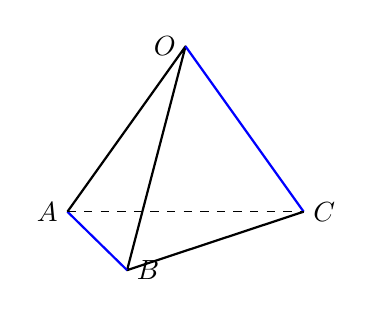
\begin{tikzpicture}[style={x={(-135:0.5)},y={(1cm,0)},z={(0,1cm)}}, line join=round, scale=3]
\coordinate[label=left: {$A$}] (A) at (0,-0.5,0);
\coordinate[label=right:{$B$}] (B) at (0.7,0,0);
\coordinate[label=right:{$C$}] (C) at (0,0.5,0);
\coordinate[label=left: {$O$}] (O) at (0,0,0.7);
\draw[thick] (A)--(O)--(B)--(C);
\draw[thick,blue] (A)--(B) (O)--(C);
\draw[dashed] (A)--(C);
\end{tikzpicture}
\end{figure}

解:
\begin{align*}
\overrightarrow{OC}\cdot \overrightarrow{AB}&=\left( \overrightarrow{AC}-\overrightarrow{AO} \right) \cdot \left( \overrightarrow{CB}-\overrightarrow{CA} \right) \\
&=\overrightarrow{AC}\cdot \overrightarrow{CB}-\overrightarrow{AO}\cdot \overrightarrow{CB}-\overrightarrow{AC}\cdot \overrightarrow{CA}+\overrightarrow{AO}\cdot \overrightarrow{CA} \\
&=\overrightarrow{AC}\cdot \overrightarrow{CB}+\overrightarrow{AC}\cdot \overrightarrow{AC}+\overrightarrow{AO}\cdot \overrightarrow{CA} \\
&=\overrightarrow{AC}\cdot \overrightarrow{AB}-\overrightarrow{AO}\cdot \overrightarrow{AC} \\
&=\overrightarrow{AC}\cdot \overrightarrow{OB}=0
\end{align*}

深入分析:

我们证明了在任意的四面体中,只要两组对棱垂直,则第三组对棱一定垂直。我们可以进一步分析,这样三组对棱垂直的情况下,四面体会有什么性质。

以$OB\bot AC$为例,意思就是$B,O$两点在$AC$上的投影重合,也即任意两个顶点在对面棱上的投影重合。根据这个结论建立如下左图的坐标系,可得:
\begin{align*}
&\because \begin{cases}
	OA\bot BC\Rightarrow \left( 0,y_A,-z_O \right) \cdot \left( -x_B,y_C,-z_B \right) =0\\
	OC\bot BA\Rightarrow \left( 0,y_C,-z_O \right) \cdot \left( -x_B,y_A,-z_B \right) =0\\
\end{cases} \\
&\therefore y_Ay_C+z_Oz_B=0
\end{align*}
四面体不一定非要正四面体,特别地,当$z_B=0$时,要么$y_A=0$要么$y_C=0$,四面体为长方体的一个角,如下右图。

\begin{figure}[h]
\centering
\begin{minipage}{.49\textwidth}
\centering
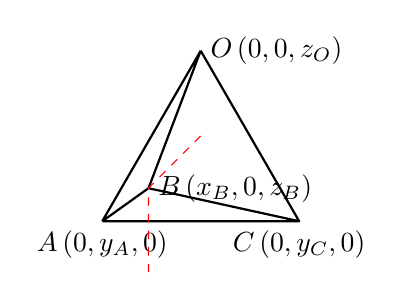
\begin{tikzpicture}[style={x={(-135:0.5)},y={(1cm,0)},z={(0,1cm)}}, line join=round, scale=2.5]
\mydrawxyz{0}{1.1}{-0.8}{0.8}{0}{1.1}
\coordinate[label=below:{$A\left( 0,y_A,0 \right) $}]   (A) at (0,-0.5,0);
\coordinate[label=below:{$C\left( 0,y_C,0 \right) $}]   (C) at (0,0.5,0);
\coordinate[label=right:{$B\left( x_B,0,z_B \right) $}] (B) at (0.75,0,0.433);
\coordinate[label=right:{$O\left( 0,0,z_O \right) $}]   (O) at (0,0,0.866);
\coordinate (Bx) at (0.75,0,0);
\coordinate (Bz) at (0,0,0.433);
\draw[thick] (O)--(A) (O)--(B) (O)--(C) (A)--(B)--(C)--(A);
\draw[dashed,red] (Bz)--(B)--(Bx);
\end{tikzpicture}
\end{minipage}
\begin{minipage}{.49\textwidth}
\centering
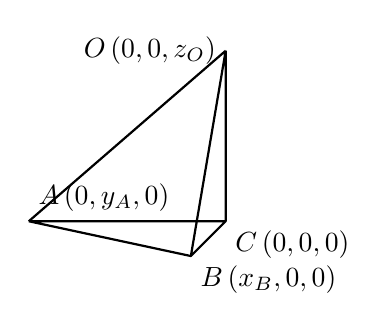
\begin{tikzpicture}[style={x={(-135:0.5)},y={(1cm,0)},z={(0,1cm)}}, line join=round, scale=2.5]
\mydrawxyz{0}{1.1}{-1.3}{0.3}{0}{1.1}
\coordinate[label=above right:{$A\left( 0,y_A,0 \right) $}] (A) at (0,-1,0);
\coordinate[label=below right:{$C\left( 0,0,0 \right) $}]   (C) at (0,0,0);
\coordinate[label=below right:{$B\left( x_B,0,0 \right) $}] (B) at (0.5,0,0);
\coordinate[label=left:       {$O\left( 0,0,z_O \right) $}] (O) at (0,0,0.866);
\draw[thick] (O)--(A) (O)--(B) (O)--(C) (A)--(B)--(C)--(A);
\end{tikzpicture}
\end{minipage}
\end{figure}

\begin{tcolorbox}
本题依然考察向量内积的几何意义。
\end{tcolorbox}

~

\begin{example}[拓广探索10,难度:$\star \star $]
如图,在四面体$OABC$中,$OA=OB,CA=CB$,$E,F,G,H$分别是$OA,OB,BC,CA$的中点。求证:四边形$EFGH$是矩形。
\end{example}

\begin{figure}[h]
\centering
\begin{tikzpicture}[style={x={(-160:0.7)},y={(1cm,-0.2cm)},z={(0,1cm)}}, line join=round, scale=2.5]
\coordinate[label=above:      {$A$}] (A) at (-0.5,-0.3,0);
\coordinate[label=left:       {$B$}] (B) at (0.5,-0.3,0);
\coordinate[label=right:      {$C$}] (C) at (0,1,0);
\coordinate[label=above:      {$O$}] (O) at (0,0,1);
\coordinate[label=left:       {$F$}] (F) at ($(O)!0.5!(B)$);
\coordinate[label=above:      {$E$}] (E) at ($(O)!0.5!(A)$);
\coordinate[label=below:      {$G$}] (G) at ($(C)!0.5!(B)$);
\coordinate[label=right:      {$H$}] (H) at ($(C)!0.5!(A)$);
\coordinate[label=above left: {$D$}] (D) at ($(A)!0.5!(B)$);
\coordinate[label=above:      {$M$}] (M) at ($(F)!0.5!(E)$);
\coordinate[label=below right:{$N$}] (N) at ($(G)!0.5!(H)$);
\draw[thick] (O)--(B)--(C)--(O);
\draw[dashed] (A)--(O) (A)--(B) (A)--(C);
\draw[thick,blue] (F)--(G);
\draw[dashed,blue] (F)--(E)--(H)--(G);
\fill[blue!50!white,opacity=0.5] (F)--(G)--(H)--(E)--cycle;
\draw[dashed,red] (O)--(D)--(C) (M)--(N);
\end{tikzpicture}
\end{figure}

解:

首先,不难通过$\overrightarrow{FG}=\overrightarrow{EH}$证明四边形$EFGH$是平行四边形。

再证明$\angle EFG$为直角。直接用向量的方法证明$\overrightarrow{FG}\cdot \overrightarrow{FE}=0$较复杂。找到$AB$中点$D$,连接$OD,CD$,不难证明$OD,CD$是三角形的中垂线,而且$FG,MN$平行且相等,所以也即证明$\overrightarrow{MN}\cdot \overrightarrow{FE}=0$。
\[
\overrightarrow{MN}\cdot \overrightarrow{FE}=\left( \overrightarrow{DN}-\overrightarrow{DM} \right) \cdot \overrightarrow{FE}=\overrightarrow{DN}\cdot \overrightarrow{GH}-\overrightarrow{DM}\cdot \overrightarrow{FE}
\]

深入分析:

不难发现,当$AB$长度一定时,$OD,CD$决定了矩形面积,我们可以考察一下当矩形面积$S$和$DO,DC$长度的关系。
\begin{align*}
&\because S=\frac{AB}{2}\cdot \frac{OC}{2} \\
&\because \cos \angle ODC=\frac{DO^2+DC^2-OC^2}{2\cdot DO\cdot DC} \\
&\therefore S=\frac{AB}{4}\cdot \left( DO^2+DC^2-2\cos \angle ODC\cdot DO\cdot DC \right)
\end{align*}
易得:
\begin{itemize}
    \item 当$S$恒定时,$OD,CD$是一个椭圆关系,可设$\angle ODC\in \left( 0,\frac{\pi}{2} \right] $,则$2\cos \angle ODC\in \left[ 0,2 \right) $,椭圆转了45°,特别地,当$DO\bot DC$时,为圆;
    \item 当$OD,CD$相互制约时,$S$有最值。
\end{itemize}

\begin{tcolorbox}
本题需要添加辅助线,用纯几何+向量的方法,事半功倍。
\end{tcolorbox}




